\documentclass[../main/main.tex]{subfiles}

\newdate{date}{18}{12}{2019}


\begin{document}

\marginpar{ \textbf{Lecture 19.} \\  \displaydate{date}. \\ Compiled:  \today.}

\section{Scaling theory}
It is used whenever you have a collective behaviour. The length scale of the problem are \( a,L,\xi  \), but  \( \xi  \) is the only relevant length scale in the problem.

Which are the experimental data which gives us this ideas? What you can see from experiment is


\begin{figure}[h!]
\centering
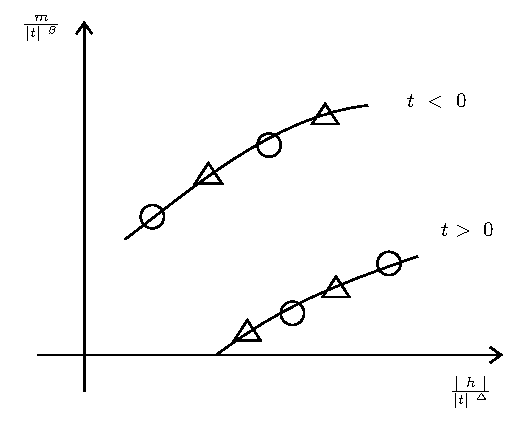
\includegraphics[width=0.6\textwidth]{../lessons/19_image/1.pdf}
\caption{\label{fig:} Description.}
\end{figure}


Widom \( \rightarrow  \) static scaling theory \( \rightarrow  \) homogeneous functions.

\subsection{Single variable \( r \) }
\( f(r) \) is homogeneous in \( r \), if \( \forall  \lambda  \in \R \) we have
\( f( \lambda r) = \lambda f(r) \). More general,
\begin{equation}
  f( \lambda r) = g (\lambda) f(r)
\end{equation}
\begin{example}
\begin{equation}
  f(r) = B r^2
\end{equation}
\begin{equation}
  f ( \lambda r) = B ( \lambda r)^2 = \lambda ^2 f (r) \quad \Rightarrow g ( \lambda ) = \lambda ^2
\end{equation}
\end{example}
Sine it is valid for any \( \lambda  \), you can choose also a \( \lambda  \) in that way
\begin{equation}
  f(r) = f (\lambda r_0) = g (\lambda ) f (r_0)
\end{equation}
\begin{theorem}[]
\begin{equation}
  g(\lambda ) = \lambda ^p
\end{equation}
where \( p \) is the degree of the homogeneity of the function.
\end{theorem}
We can make it for any variable, not only for a single one.

\subsection{Generalized homogeneous functions}
We are discussing \( f(x,y) \), that is a generalized homogeneous function if \( f (\lambda ^a x, \lambda ^b y) = \lambda f(x,y)\). In general any polynomial is a generalized homogeneous function.
If we choose \( \lambda ^p \equiv s \), we have
\begin{equation}
  f ( s^{a/p} x, s^{b/p} y) = s f(x,y)
\end{equation}

Consider \( t \equiv  \frac{T - T_c}{T_c}, h = \frac{H - H_c}{H_c} \)
\begin{equation}
  f (T,H) = f_{ANA} (T,H) + f_{SING} (t,h)
\end{equation}
where \( f_{ANA} \) is an analytic term and \( f_{SING} \) diverges, has a singularity.

The singular part of the free energy
\begin{equation}
  f_s ( \lambda ^{p_1} t, \lambda ^{p_2} h) = \lambda f_s (t,h)
\end{equation}
where \( \forall \lambda \in \R \).

Another important feature, choose \( \lambda  \) as
\begin{equation}
  \lambda = h^{-1/p_2} \quad \Rightarrow f_s (t,h) = h^{1/p_2} f_s (h^{-p_1/p_2} t , 1)
\end{equation}
\begin{equation}
  \Delta  \equiv \frac{p_1}{p_2}
\end{equation}
is called the \emph{gap exponent}.

\( M \) is the first derivative of \( f \) with respect to \( H \).
\begin{equation}
  \lambda ^{p_2} M_s ( \lambda ^{p_1} t, \lambda ^{p_2} h) = \lambda M_s (t,h)
\end{equation}
so you have the same story for the magnetization.
Consider \( h=0 \) and \( t \rightarrow 0^- \), we have
\begin{equation}
  M_s (t) \sim (-t)^{\beta }
\end{equation}
starting from this one try to figure out what is happening at this level.
\begin{equation}
  M_s (t,0) = \lambda ^{p_2 -1} M_s ( \lambda ^{p_1} t,0)
\end{equation}
\begin{equation}
  \lambda ^{p_1} t = -1 \quad \Rightarrow \lambda = (t)^{-1/p_1}
\end{equation}
so
\begin{equation}
  M_s (t,0) = - (t)^{\frac{1-p_2}{p_1}} M_s (-1,0)
\end{equation}
\begin{equation}
  \beta = \frac{1-p_2}{p_1}
\end{equation}
For \( \delta  \), we have  \( T=T_c \) and \( h \rightarrow 0^+ \), so the magnetization goes like \( M_s \sim h^{1/\delta } \).
\begin{equation}
  M_s (0,h) = \lambda ^{p_2 - 1} M_s (0,\lambda ^{p_2} h)
\end{equation}
Now we want
\begin{equation}
  \lambda ^{p_1} h = 1 \quad \Rightarrow \lambda = h ^{-1/p_2}
\end{equation}
\begin{equation}
  M_s (0,h) = h ^{\frac{1-p_2}{p_2}} M_s (0,+1)
\end{equation}
\begin{equation}
  \delta = \frac{p_2}{ 1 - p_2 }
\end{equation}
From this you have a very simple relation
\begin{equation}
  p_1 = \frac{1}{\beta (\delta +1)}, \quad p_2 = \frac{\delta }{\delta + 1}
\end{equation}
\begin{equation}
  \frac{p_2}{p_1} = \Delta = \beta \delta
\end{equation}

Our relations are
\begin{equation}
  f_s (\lambda ^{p_1} t, \lambda ^{p_2} h) = \lambda f_s (t,h)
\end{equation}
\begin{equation}
  M_s (t,h) = \lambda ^{p_2 - 1} M_s (\lambda ^{p_1} t, \lambda ^{p_2} h)
\end{equation}
We have \( \lambda = \abs{t}^{-1/p_1}  \)
\begin{equation}
  M_s (t,h) = \abs{t}^{\frac{1-p_2}{p_1}} M_s ( \frac{t}{\abs{t} }, \frac{h}{\abs{t}^{\Delta } })
\end{equation}
\begin{equation}
  \frac{M_s (t,h)}{\abs{t}^{\beta } } = M_s ( \frac{t}{\abs{t} }, \frac{h}{\abs{t}^{\Delta } })
\end{equation}

By using these hypothesis you can get equalities. All the inequality that you have in thermodynamics becames equalities.
In particular, we have the Griffit relation
\begin{equation}
  \alpha + \beta (\delta +1) = 2
\end{equation}
and the Rushbrooks relation
\begin{equation}
  \alpha + 2 \beta + \gamma = 2
\end{equation}

\section{Kadanoff 1966}
How can we relate the coupling costant of the two hamiltonian. This is the idea of the renormalization group.
\begin{equation}
  - \beta \mathcal{H}_{\Omega } = k \sum_{\expval{ij} }^{} \sigma _i \sigma _j + h \sum_{i}^{} \sigma _i
\end{equation}
with
\begin{equation}
  \sigma _i = \pm 1, \quad k \equiv \frac{J}{k_B T}, \quad h \equiv \frac{H}{k_B T}
\end{equation}
we assume
\begin{equation}
  r \ll \xi  \quad \Rightarrow a \ll l a \ll \xi (t)
\end{equation}
We can build up many procedure.
This is the \emph{Block spin transformation}, the idea is divide into cell of length \( la \) (figure 2) and we replace it with (figure 3).

\begin{equation}
  S_I \equiv \frac{1}{\abs{m_l} } \frac{1}{l^D} \sum_{i \in I}^{}  \sigma _i
\end{equation}
with the sum is over all the sites with a given cell.
Define the magnetization
\begin{equation}
  m_l \equiv \frac{1}{l^D} \sum_{i \in I}^{} \sigma _i
\end{equation}

The frist assumption is that the Hamiltonian of the new system \( \mathcal{H}_l \) is equal in form to \( \mathcal{H}_ \Omega  \). It means that we can write
\begin{equation}
  - \beta \mathcal{H}_l = k_l \sum_{\expval{IJ} }^{} S_I S_J  + h_l \sum_{I}^{} S_I
\end{equation}

\begin{equation}
  N_l = \frac{N}{l^D}
\end{equation}
How you measure in the new system the lengths? the correlations lengths. Before we have changed the size of the system. We have increased the ruler, so the number is smaller now. It seems stupid but it is fundamental.
\begin{equation}
  \xi _l = \frac{\xi }{l}
\end{equation}
were the last relation it is very important!

Anyway for the Kadanoff it does not meant so much because we do not iterate.
The new distance of the critical point in the new system \( t_l \) is
\begin{equation}
  t_l > t
\end{equation}

We have
\begin{equation}
  h \sum_{i}^{} \sigma _i = h \sum_{I}^{} \sum_{i \in \sigma _i}^{}  \sigma _i = h \sum_{I}^{}    \abs{m_l} l^D S_I
  = \underbrace{h \abs{m_l} l^D}_{h_l} \sum_{I}^{} S_I
\end{equation}
\begin{equation}
  h_l = \abs{m_l} l^D h
\end{equation}

What happens to the free energy?
Since \( h_l \) is equal in form to \( h \), the story is the same. So also for the free energy there would be a difference in the number of spins.

If I take \(   N_l f_s (t_l,h_l) \) this is equal to
\begin{equation}
  N_l f_s (t_l,h_l) = N f_s (t,h)
\end{equation}
\begin{equation}
  \Rightarrow  f_s (t_l,h_l) = l^D f_s (t,h)
\end{equation}

Somehow we are getting just for free \( \lambda \equiv l^D \). Now we need other assumptions. The second assumption is
\begin{equation}
  t_l = t l^{Y_t} \quad h_l = h l^{Y_h}
\end{equation}
\begin{equation}
  f_s (t,h) = l^{-D} f_s (t l^{Y_t}, h l^{Y_h})
\end{equation}
Let us take \( l= \abs{t}^{-1/Y_t}  \)
\begin{equation}
  f_s (t,h) = \abs{t}^{D/Y_t} f_s (1, h \abs{t}^{-Y_h/Y_t} )
\end{equation}
\begin{equation}
  \Delta = \frac{Y_h}{Y_t} \quad \Rightarrow 2 - \alpha = \frac{D}{Y_t}
\end{equation}
We are changing the ruler
\begin{equation}
  G_{IJ} (\va{r}_l, t_l) \equiv \expval{S_I S_J} - \expval{S_I}\expval{S_J}
\end{equation}
\begin{equation}
  \abs{\va{r}_l} = \frac{\va{r}}{l}
\end{equation}
We want to write \( G_{IJ} \) for \( \sigma _i \sigma _j \), what we get at the end is
\begin{equation}
  G_{IJ} (\va{r}_l, t_l) = l^{2(D-Y_h)} G_{ij} (\va{r},t)
\end{equation}

What we get resclaing the system is
\begin{equation}
  G_{IJ} \qty(\va{r}/l, t l ^{Y_t}, h l^{Y_h}) l^{2(D-Y_h)} G_{ij} (\va{r},t)
\end{equation}
\begin{equation}
  l = t^{-1/Y_t}
\end{equation}
\begin{equation}
  G_{IJ} (\va{r} t^{1/Y_t}, 1, h t^{-Y_h/Y_t}) = t^{-2 \frac{D- Y_h}{Y_t}} G_{ij} (\va{r},t)
\end{equation}





\end{document}
